\documentclass[journal]{IEEEtran}
\usepackage{amsmath,amsfonts}
\usepackage{algorithmic}
\usepackage{algorithm}
\usepackage{array}
\usepackage[caption=false,font=normalsize,labelfont=sf,textfont=sf]{subfig}
\usepackage{textcomp}
\usepackage{url}
\usepackage{verbatim}
\usepackage{graphicx}
\usepackage{cite}
\usepackage[T1]{fontenc}
\usepackage[hungarian]{babel}
\usepackage{booktabs}


\begin{document}

\title{Madárfajok azonosítása hangfelvételek alapján\\CNN alkalmazásával (BirdCLEF challenge)}

\author{
  \IEEEauthorblockN{Agócs Norbert, Magyari Zsombor, Vas Benedek Zoltán}\\[0.5em]
  \IEEEauthorblockN{Budapesti Műszaki és Gazdaságtudományi Egyetem}
}

\markboth{Deep Learning a gyakorlatban Python alapon | 2025/26/1}%
{Agócs N, Magyari Zs, Vas B.: Madárfajok azonosítása hangfelvételek alapján CNN alkalmazásával (BirdCLEF challenge)}

\maketitle

\begin{abstract}
  A jelen projekt a BirdCLEF kihívás keretében végzett deep learning alapú madárhang-osztályozási feladatot mutatja be. A cél egy olyan automatikus felismerőrendszer megvalósítása, amely rövid hangfelvételek alapján képes a madárfajok azonosítására. A megközelítés alapját a hangjelek idő--frekvencia reprezentációja és egy korszerű konvolúciós neurális hálózat (CNN) képezi.
\end{abstract}

\begin{IEEEkeywords}
  Machine Learning, Deep Learning, Convolutional Neural Networks, Audio Pattern Recognition, Audio Classification, BirdCLEF, Python, Keras, TensorFlow
\end{IEEEkeywords}

% Parancsok
% \url{http://tug.ctan.org/info/lshort/english/lshort.pdf}
% Idézőjel: ``text''
% \IEEEPARstart{T}{his}
%  \cite{ref1}

% \begin{figure}[!t]
%   \centering
%   
\includegraphics[width=2.5in]{fig1}
%   \caption{Simulation results for the network.}
%   \label{fig_1}
% \end{figure}

% \begin{figure*}[!t]
%   \centering
%   \subfloat[]{
\includegraphics[width=2.5in]{fig1}%
%   \label{fig_first_case}}
%   \hfil
%   \subfloat[]{
\includegraphics[width=2.5in]{fig1}%
%   \label{fig_second_case}}
%   \caption{Dae. Ad quatur autat ut porepel itemoles dolor autem fuga. Bus quia con nessunti as remo di quatus non perum que nimus. (a) Case I. (b) Case II.}
%   \label{fig_sim}
% \end{figure*}

% \begin{algorithm}[H]
%   \caption{Weighted Tanimoto ELM.}\label{alg:alg1}
%   \begin{algorithmic}
%     \STATE {\textsc{PREDICT}}$(\mathbf{X} )$
%     \STATE \hspace{0.5cm}$ \mathbf{H} \gets  (\mathbf{X}^T\textbf{W} )/( \mathbb{1}\mathbf{X}  + \mathbb{1}\textbf{W}- \mathbf{X}^T\textbf{W}  ) $
%     \STATE \hspace{0.5cm}\textbf{return}  $\textsc{sign}( \mathbf{H} \beta )$
%   \end{algorithmic}
%   \label{alg1}
% \end{algorithm}

\section{Bevezetés}
  
  \IEEEPARstart{A}{} madarak mindenki számára jól ismert élőlények, hiszen a Föld valamennyi élőhelyén jelen vannak. Az élőlények, így különösen a madárfajok azonosítása régóta a tudományos kutatások középpontjában áll. Míg a madarak megkülönböztetése külső megjelenésük alapján megfelelő előképzettséggel viszonylag könnyen megvalósítható, addig hangjuk alapján történő felismerésük lényegesen nagyobb kihívást jelent.
  
  A madárhangok elemzése és azonosítása kiemelt szerepet tölt be a biodiverzitás monitorozásában, a fajok elterjedésének és vándorlási mintázatainak nyomon követésében, valamint a természetvédelmi kutatások támogatásában. A nagymennyiségű, hosszú időtartamú akusztikai felvételek feldolgozása ugyanakkor összetett feladat, amely a változó környezeti és zajviszonyok miatt robusztus és adaptív módszereket igényel. Az utóbbi években a deep learning területén elért eredmények jelentős előrelépést hoztak az automatikus hangfelismerésben. A jelen projekt célja egy konvolúciós neurális hálózaton (CNN) alapuló megközelítés bemutatása, amely alkalmas nagyléptékű madárhang-osztályozási feladatok megoldására.

\section{Tématerület ismertetése,\\korábbi megoldások}
  
  A madárhangok automatikus felismerése régóta vizsgált problémakör a bioakusztika és a jelfeldolgozás határterületén. A deep learning módszerek megjelenése előtt a megoldások túlnyomó többsége kézzel tervezett akusztikai jellemzőkre épült, mint például a mel-frekvencia alapú cepstrális együtthatók (MFCC), spektrális energiaeloszlások és időbeli statisztikák. Ezeket a jellemzőket hagyományos osztályozó algoritmusokkal -- többek között support vector machines (SVM) és k-nearest neighbors (k-NN) módszerekkel -- kombinálták.  Bár ezek a megközelítések kontrollált környezetben elfogadható eredményeket mutattak, teljesítményük jelentősen romlott zajos, természetes hangképek esetén, valamint korlátozott volt az általánosíthatóságuk összetett mintázatokra. \cite{nilanjana2021}

  A konvolúciós neurális hálózatok (CNN) elterjedése alapvető szemléletváltást hozott a hangfelismerési feladatok megközelítésében. A hangjeleket kétdimenziós idő--frekvencia tartományban, elsősorban mel-spektrogramok formájában dolgozták fel. Ez lehetővé tette az audioosztályozás képfeldolgozási problémaként való kezelését. A korai CNN-alapú megoldások igazolták, hogy a tanult jellemzők robusztusabbak a háttérzajjal és a fajon belüli eltérésekkel szemben, mint a hagyományos, kézzel definiált jellemzőkre épülő módszerek \cite{Grill2017, lasseck2018, kahl2018}.

  A hálózatok mélységének növekedésével párhuzamosan az általános képfeldolgozás területén sikeresen alkalmazott architekturális újítások a hangfeldolgozás területén is megjelentek. A reziduális kapcsolatokra épülő ResNet architektúra jelentősen javította a mély neurális modellek taníthatóságát és numerikus stabilitását \cite{he2015}, míg a sűrűn csatolt konvolúciós struktúrák hatékonyabb tanítást és a jellemzők eredményesebb felismerését tették lehetővé \cite{huang2018}. Ezek az architektúrák adták a nagy teljesítményű madárhang-felismerő rendszerek alapját.

  Az összetett hangfelvételek feldolgozása új kihívásokat vetett fel, különösen az egymást átfedő hangesemények kezelése szempontjából. E problémák kezelésére számos tanulmány modell-együtteseken (\emph{ensebmle}) alapuló megközelítéseket, kiterjedt adatbővítési (\emph{data augmentation}) stratégiákat, valamint célzott utófeldolgozást alkalmazott a hamis pozitív detektálások számának csökkentése érdekében \cite{conde2021, kahl2021}. Az így elért eredmények rámutattak arra, hogy a rendszer teljesítményét nem kizárólag a neurális hálózati architektúra határozza meg, hanem a teljes feldolgozási lánc kulcsszerepet játszik.

  A ritka madárfajok esetén tapasztalt egyenlőtlen adateloszlások kezelése érdekében a kutatások egyre nagyobb hangsúlyt helyeztek a kis mintás megközelítésekre, valamint az átvitt tanulásra (\emph{transfer learning}). Az előre betanított modellek alkalmazása lehetővé tette egy stabilabb jellemzőtér kialakítását még kis mintás tanítóadatok esetén is \cite{conde2022, miyaguchi2022}. Ezt az irányvonalat tovább erősítették a részlegesen felügyelt tanulási módszerek (semi-supervised learning) és az álcímkézésen alapuló eljárások (\emph{pseudo-labeling}) alkalmazása \cite{miyaguchi2023, miyaguchi2024}.

  A legújabb kutatások a számítási hatékonyság és a gyakorlati alkalmazhatóság javítására összpontosítanak. Ennek egyik iránya a hatékonyabb architektúrák alkalmazása, mint például az \emph{EfficientNet} \cite{tan2021}. Ezzel párhuzamosan megjelentek a tokenizált spektrogram-alapú megközelítések, valamint az önfelügyelt tanulási eljárások (\emph{self-supervised learning}), amelyek nagy mennyiségű címkézetlen adat hatékony hasznosítását teszik lehetővé \cite{miyaguchi2025}. Továbbá olyan módszerek is megjelentek, amelyek a frekvencia explicit beágyazásával törekednek a hasonló akusztikus motívumok megkülönböztetésére \cite{r2025}.


\section{Módszertan}

  Az alkalmazott módszertan három fő lépésből áll: a hangfelvételekből spektrogramok állítunk elő, létrehozunk egy konvolúciós neurális hálózatot, majd a spektrogrammok alapján tanítjuk. A hangfelismerési feladatot képfeldolgozási problémaként kezeljük. A betanított modellt végül egy elkülönített felvételeket tartalmazó teszt adathalmazon értékeljük.

  \subsection{Adathalmaz}

    A madárfajok hangalapú azonosításának megvalósításához a BirdCLEF 2024 adathalmazt használjuk. Az adathalmaz összesen 24.459 rövid, címkézett \texttt{.ogg} formátumú hangfelvételt tartalmaz, amelyek 182 különböző madárfajhoz kapcsolódnak. A felvételek a Xeno-Canto adatbázisból származnak, ennek következtében a hanganyagok jelentős változatosságot mutatnak mind a környezeti zajszint, mind a felvételi minőség tekintetében. A \texttt{train\_metadata.csv} fájl minden hangfelvételhez strukturált metaadatokat biztosít (Táblázat \ref{tab:metadata}), többek között a hangfájlhoz rendelt fajazonosítót, a felvétel készítésének földrajzi helyét, valamint a hangfájl nevét. A hangfelvételek egységes, 32 kHz-es mintavételezési frekvenciával, monó csatornán kerültek rögzítésre. Az egyes hangfájlokhoz társított madárfaj nem feltétlenül van jelen a teljes felvétel időtartama alatt, illetve nem kizárólagosan fordul elő benne.

    \begin{table}[h]
      \centering
      \caption{Példa a \texttt{train\_metadata.csv} állomány felépítésére}
      \label{tab:metadata}
      \begin{tabular}{llll}
        \toprule
        \textbf{Mező} & \textbf{Típus} & \textbf{Példa} & \textbf{Leírás} \\
        \midrule
        primary\_label & string & asbfly & Fajazonosító \\
        type & list & [call], [song] & Hangtípus \\
        latitude & float & 39.2297 & Szélesség \\
        longitude & float & 118.1987 & Hosszúság \\
        common\_name & string & Asian Brown Flycatcher & Név \\
        rating & float & 5.0 & Minőség \\
        filename & string & asbfly/XC134896.ogg & Hangfájl neve \\
        \bottomrule
      \end{tabular}
    \end{table}

    A BirdCLEF adathalmaz egy nyilvános Google Drive mappában található, ahonnan a fájlok automatikusan történik. 

  \subsection{Adatfeldolgozás}

    A hangfájlok betöltése és feldolgozása a \texttt{librosa} könyvtár segítségével történik, egységes, a megadott $f_s = 32 \, \textrm{kHz}$ mintavételezési frekvencia alkalmazásával. Az előfeldolgozás során minden hangfelvételt egységes, 15 másodperces hosszra alakítunk: a hosszabb felvételeket levágjuk, míg a rövidebbeket nullával töltjük fel. A nyers hangjelekből ezt követően mel-skálázott spektrogramokat állítunk elő rövid idejű Fourier-transzformáció (STFT) alkalmazásával. 
    
    A mel-spektrogram olyan idő--frekvencia ábrázolás, amely a hangjel energiájának eloszlását jeleníti meg az idő és a frekvencia függvényében, az emberi hallás frekvenciaérzékeléséhez igazított skálán. A spektrogram frekvenciatengelye hagyományosan lineáris skálán van értelmezve, azonban az emberi hallás frekvenciafelbontása nem lineáris. A Hertz- és mel-skála közötti kapcsolatot az alábbi összefüggés írja le:
    \begin{equation}
      m(f) = 2595 \cdot \log_{10}\left(1 + \frac{f}{700}\right),
    \end{equation}
    ahol $f$ a frekvencia Hertzben, $m(f)$ pedig a megfelelő mel-skálázott frekvenciaérték. A frekvenciatartományt 20 Hz és 16 kHz közé korlátozzuk (emberi érzékelés tartománya), amely lefedi a madárhangok elemzése szempontjából releváns akusztikus tartományt. A kapott mel-spektrogrammot decibel-skálára alakítjuk, majd mintánként normalizáljuk a [0,1] intervallumba a \emph{Min--Max} módszer alkalmazásával:
    \begin{align}
      S_{\mathrm{dB}} &= 10 \cdot \log_{10} \left( \frac{S}{P_{\mathrm{ref}}} \right), \\
      S_{\mathrm{norm}} &= \frac{S_{\mathrm{dB}} - \min(S_{\mathrm{dB}})}{\max(S_{\mathrm{dB}}) - \min(S_{\mathrm{dB}})},
    \end{align}
    ahol $S$ a mel-spektrogram értéke, a $P_{\mathrm{ref}} = 1.0$ referenciaérték. Az így előállított és normalizált mel-spektrogram rögzített méretű, kétdimenziós, $128 \times 384$ px méretű, képalapú bemenetként szolgál a konvolúciós neurális hálózat számára, lehetővé téve az idő--frekvencia mintázatok hatékony tanulását a képfeldolgozási problémaként. A madárhangok hullámformájára és mel-spektrogramjára egy példa \aref{fig_1}. ábrán látható.
    \begin{figure}[!h]
      \centering
      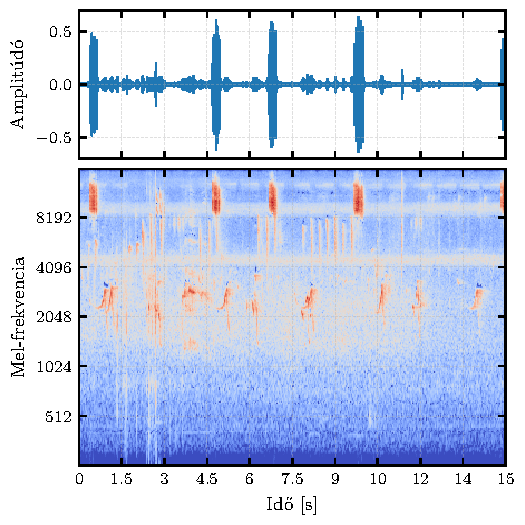
\includegraphics[width=\linewidth]{figures/fig1.pdf}
      \caption{Példa egy hangfelvétel hullámformájára és mel-spektrogramjára.}
      \label{fig_1}
    \end{figure}

  \subsection{Neurális hálózat architektúra}

    TODO

  \subsection{Tanítási folyamat}

    TODO

  \subsection{Kiértékelés}
    
    TODO

\section{Eredmények}

  TODO

\section{Összefoglalás} % + Jövőbeli tervek

  TODO



% {\appendix[Proof of the Zonklar Equations]
% Use $\backslash${\tt{appendix}} if you have a single appendix:
% Do not use $\backslash${\tt{section}} anymore after $\backslash${\tt{appendix}}, only $\backslash${\tt{section*}}.
% If you have multiple appendixes use $\backslash${\tt{appendices}} then use $\backslash${\tt{section}} to start each appendix.
% You must declare a $\backslash${\tt{section}} before using any $\backslash${\tt{subsection}} or using $\backslash${\tt{label}} ($\backslash${\tt{appendices}} by itself
% starts a section numbered zero.)}

%{\appendices
%\section*{Proof of the First Zonklar Equation}
%Appendix one text goes here.
% You can choose not to have a title for an appendix if you want by leaving the argument blank
%\section*{Proof of the Second Zonklar Equation}
%Appendix two text goes here.}


% References
\newpage
\bibliographystyle{ieeetran}
\bibliography{references}


\vfill

\end{document}


